\Gls{ppo} is a more efficient and stable algorithm than \gls{dqn}, and it
is able to learn the optimal policy faster. \gls{ppo} is a policy-based
algorithm, which means that it learns the optimal policy directly, rather
than learning the optimal value function. This makes it more efficient, as
it does not have to learn the value function first, and it is also more
stable, as it does not have to deal with the issues surrounding the
Q-values exploding.

\Gls{ppo} is based on the idea of optimizing the policy by taking small
steps in the direction of the gradient of the policy, and then updating
the policy using the gradient of the policy. This is done by using the
policy gradient theorem, which states that the gradient of the policy is
equal to the gradient of the log-probability of the action multiplied by
the advantage function. The advantage function is the difference between
the value function and the Q-value function, and it represents how much
better the action is than the average action.

\begin{algorithm}[H]
    \caption{Proximal Policy Optimization}
    \label{alg:ppo}
    \begin{algorithmic}
        \State Initialize policy $\pi_{\theta}$ with random weights $\theta$
        \State Initialize value function $V_{\phi}$ with random weights $\phi$
        \State Initialize environment $E$
        \For{iteration = 1, 2, ...}
            \State Collect trajectories $\tau$ using policy $\pi_{\theta}$
            \State Compute advantages $A^{\pi_{\theta}}$
            \State Optimize policy by taking small steps in the direction of the gradient of the policy
            \State Update policy using the gradient of the policy
            \State Optimize value function by taking small steps in the direction of the gradient of the value function
            \State Update value function using the gradient of the value function
        \EndFor
    \end{algorithmic}
\end{algorithm}

\subsection{Results}\label{subsec:agent-ppo-results}
Our initial results are from our own implementation of \gls{ddqn} with
a learning rate of 0.001, a discount factor of 0.99, and a batch size of 32.
The neural netowrk has two hidden layers with 1024 units each and uses the
ReLU activation function. The target network is updated every 1000 steps,
and prioritized experience replay is used with $\alpha = 0.6$ and
$\beta = 0.4$.

\begin{figure}[H]
    \begin{subfigure}{0.45\textwidth}
        \centering
        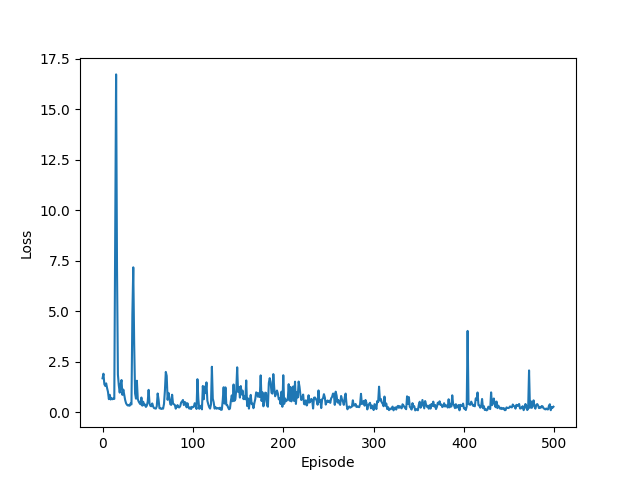
\includegraphics[width=\textwidth]{img/ddqn-500-loss.png}
        \caption{Loss over 500 episodes}
        \label{fig:ddqn-500-loss}
    \end{subfigure}
    \begin{subfigure}{0.45\textwidth}
        \centering
        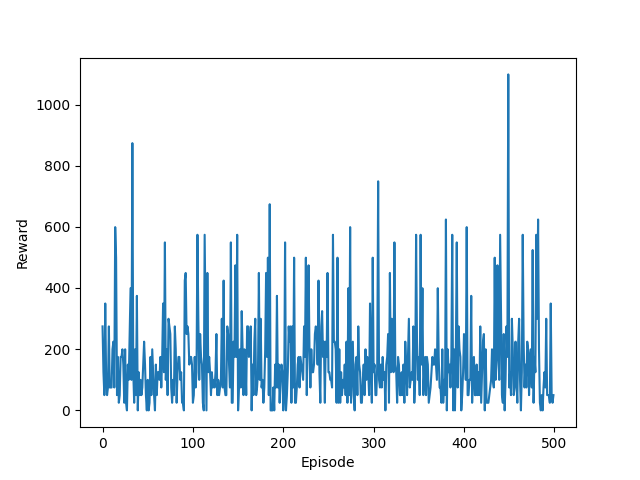
\includegraphics[width=\textwidth]{img/ddqn-500-reward.png}
        \caption{Reward over 500 episodes}
        \label{fig:ddqn-500-reward}
    \end{subfigure}
    \caption{Double DQN training results}
    \label{fig:ddqn-500}
\end{figure}

As we can see in \cref{fig:ddqn-500}, the loss converges to a value of
approximately 0.5, but the reward does not seem to improve significantly.
This is also confirmed through testing, where the agent simply seems to move
to the left, jumping off and dying. This could be due to several reasons,
all of which mentioned previously in \cref{ch:environment}.

Training the agent for 1600 episodes, we see a similar pattern, followed
by a very unusual spike in the loss, as seen in \cref{fig:ddqn-2000-1600-loss}.

\begin{figure}[H]
    \begin{subfigure}{0.45\textwidth}
        \centering
        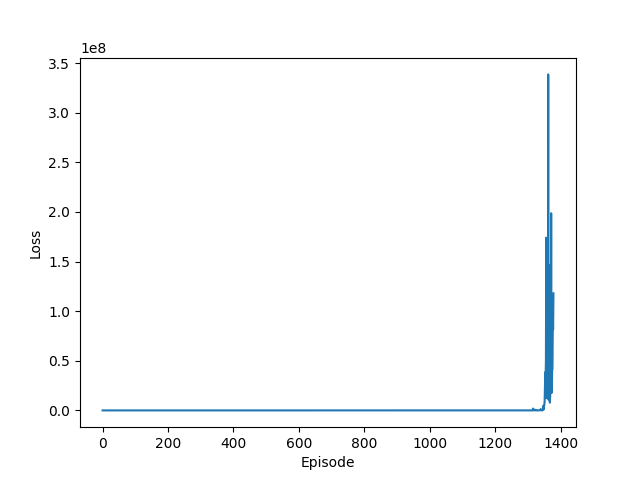
\includegraphics[width=\textwidth]{img/ddqn-2000-1600-loss.png}
        \caption{Loss over 1600 episodes}
        \label{fig:ddqn-2000-1600-loss}
    \end{subfigure}
    \begin{subfigure}{0.45\textwidth}
        \centering
        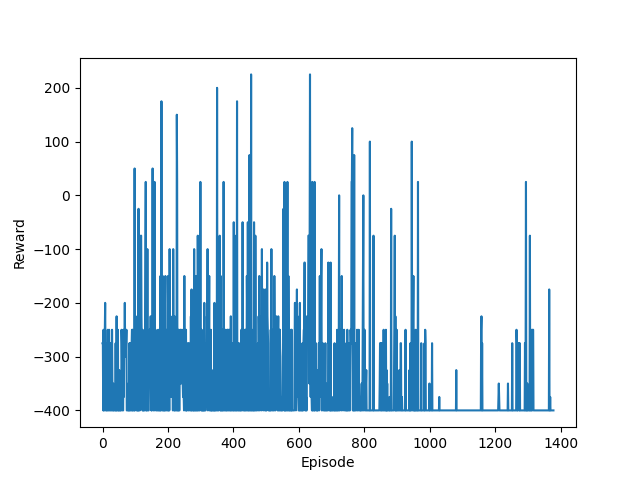
\includegraphics[width=\textwidth]{img/ddqn-2000-1600-reward.png}
        \caption{Reward over 1600 episodes}
        \label{fig:ddqn-2000-1600-reward}
    \end{subfigure}
    \caption{Double DQN training results}
    \label{fig:ddqn-2000-1600}
\end{figure}

Here, we see that the loss remains low, but then suddenly increases into the
billions. This is likely due to the Q-values exploding, which is a common
problem in \gls{rl} algorithms. We can combat this by using gradient clipping,
which limits the size of the gradients, or by using a different architecture
for the neural network.

Another point to consider is the training speed. Even with a strong GPU, the
training process is very slow, and it is difficult to experiment with different
hyperparameters. This is why we have chosen to use Stabe Baselines 3, which
provides a more efficient implementation of the algorithms.

Using the a learning rate of 0.0001, and having implemented all of the
improvements mentioned in \cref{ch:environment}, we trained a \gls{dqn} agent
for 40 million steps. The results can be seen in \cref{fig:dqn}.

\begin{figure}[H]
    \begin{subfigure}{0.45\textwidth}
        \centering
        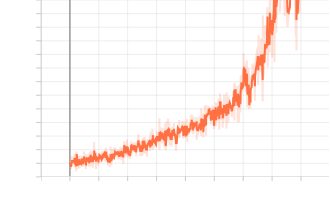
\includegraphics[width=\textwidth]{img/dqn_len_mean.png}
        \caption{Mean episode length}
        \label{fig:dqn_len_mean}
    \end{subfigure}
    \begin{subfigure}{0.45\textwidth}
        \centering
        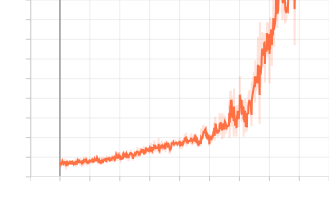
\includegraphics[width=\textwidth]{img/dqn_rew_mean.png}
        \caption{Mean episode reward}
        \label{fig:dqn_reward_mean}
    \end{subfigure}
    \caption{DQN training results}
    \label{fig:dqn}
\end{figure}

As we can see in \cref{fig:dqn}, the agent is able to learn to play the game
quite well, with the mean episode length and the mean episode reward increasing 
steadily. Also through testing, the agent is able to complete several levels
of the game, which is a significant improvement over the previous results.

However, the agent still has some issues. It is not able to complete the game
consistently, and it still has a tendency to jump off the platform and die.
This could be due to the fact that the agent is not able to learn the optimal
policy, or that the environment is too complex for the agent to learn. It could
also be due to the factors surrounding the number of lives mentioned in
\cref{sec:environment-termination}.

Although it may be interesting to continue training the agent, we have chosen
to move on to the next algorithm, \gls{ppo}, as it is more efficient and
provides better results in general.